\documentclass[12 pt, russian]{article}
\usepackage[T1]{fontenc}
\usepackage{ulem}
\usepackage[utf8]{luainputenc}
\usepackage{geometry}
\usepackage[pdftex]{graphicx}
\geometry{verbose,tmargin=3cm,bmargin=3cm,lmargin=3cm,rmargin=3cm}
\usepackage{amstext}
\usepackage{amsthm}
\usepackage{amssymb}
\usepackage{amsmath}
\usepackage[T1,T2A]{fontenc}
\usepackage[utf8]{inputenc}
\usepackage[english,main=russian]{babel}
\usepackage{setspace}
\usepackage{esint}
\usepackage{comment}
\usepackage{babel}
\usepackage{float}
\usepackage{amsfonts}
\usepackage{fullpage} 
\usepackage{parskip} 
\usepackage{tikz} 
\usepackage{indentfirst}

\def\hbr{\hfil\break}
\newcommand\F{\mbox{I\kern-2pt F}}
\newcommand\cA{{\cal A}}
\newcommand\cE{{\cal E}}
\newcommand\cC{{\cal C}}
\newcommand\cF{{\cal F}}
\newcommand\cG{{\cal G}}
\newcommand\cI{{\cal I}}
\newcommand\cK{{\cal K}}
\newcommand\cL{{\cal L}}
\newcommand\cB{{\cal B}}
\newcommand\cN{{\cal N}}
\newcommand\cM{{\cal M}}
\newcommand\cX{{\cal X}}
\newcommand\cD{{\cal D}}
\newcommand\cO{{\cal O}}
\newcommand\cR{{\cal R}}
\newcommand\cP{{\cal P}}
\newcommand\cQ{{\cal Q}}
\newcommand\cS{{\cal S}}
\newcommand\cT{{\cal T}}
\newcommand\cV{{\cal V}}
\newcommand\cY{{\cal Y}}
\newcommand\cZ{{\cal Z}}
\newcommand\R{\bbr}
\newcommand\uv{{\underline v}}
\newcommand\uw{{\underline w}}
\newcommand\up{{\underline p}}
\newcommand\uV{{\underline V}}
\newcommand\uW{{\underline W}}
\newcommand\bp{{\bar p}}
\newcommand\bv{{\bar v}}
\newcommand\bw{{\bar w}}
\newcommand\bV{{\bar V}}
\newcommand\bW{{\bar W}}
\def\bbr{{\mathbb R}}
\def\bbn{{\mathbb N}}
\def\bbc{{\mathbb C}}
\def\bbz{{\mathbb Z}}
\newcommand\e{{\varepsilon}}
\newtheorem{theo}{Theorem}[section]
\newtheorem{prop}[theo]{Proposition}
\newtheorem{lemm}[theo]{Lemma}
\newtheorem{coro}[theo]{Corollary}
\newtheorem{defin}[theo]{Definition}
\newtheorem{rem}[theo]{Remark}
\newcommand\fdem{$\Box$}
\newcommand\beq{\begin{equation}}
\newcommand\eeq{\end{equation}}
\newcommand\bea{\begin{eqnarray}}
\newcommand\eea{\end{eqnarray}}
\newcommand\bean{\begin{eqnarray*}}
	\newcommand\eean{\end{eqnarray*}}


\title{Курсовая работа ФИО}
\raggedbottom
\begin{document}
\thispagestyle{empty}
\newtheorem{Thm}{Теорема}[section]
\newtheorem{Lem}{Лемма}[section]
\newtheorem{Rem}{Замечание}[section]
\newtheorem{Co}{Следствие}[section]
\theoremstyle{definition}
\newtheorem{Exam}{Пример}[section]
\newtheorem{Dfn}{Определение}[section]
\sloppy
\begin{titlepage}
\begin{center}
Московский государственный университет имени~М.~В.~Ломоносова\\
Механико-математический факультет\\
Кафедра Теории Вероятностей\\
\centering
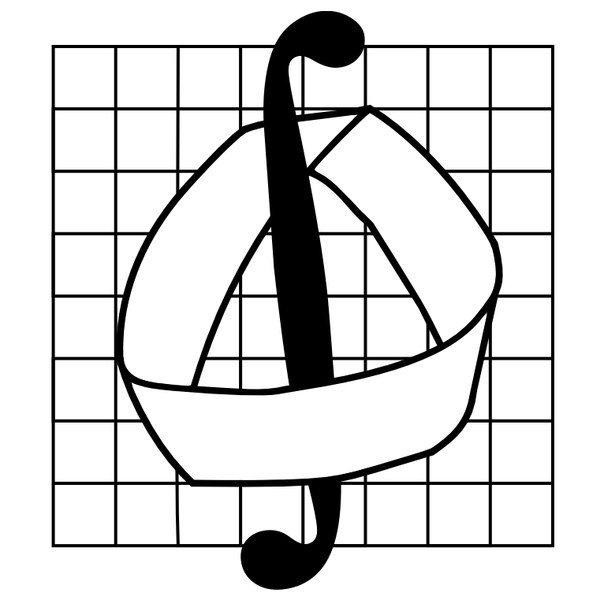
\includegraphics[width=0.3\textwidth]{mechmath.jpg}

\vspace*{100pt} Отчёт\\
студента 409 группы \\
Сидоренко Артура Павловича \\
\vspace{10pt} {\Large{\textbf{}}\\}
\textbf{Численное решение одного уравнения второго порядка}
\vspace*{40pt}


\vspace*{\fill} Москва, 2020
\end{center}
\end{titlepage}

\section{Постановка задачи}
Дана краевая задача
\beq
\label{task}
-u''(x) + b(x) u(x) = f(x), u(0) = 0, u'(1) = 0.
\eeq

Требуется составить разностную схему для поиска решения задачи на отрезке $[0, 1]$ и численно её апробировать. Предлагается использовать смещённую вправо сетку на $[0, 1]$ из $N$ узлов с шагом $h = 2 / (2N - 1)$,  $x_k = kh$. 


\section{Разностная схема}

Я буду руководствоваться определениями в \cite{Kornev1}, стр. 254-259 и \cite{Kornev2}, стр.27-32.

Предложим следующую разностную схему:
\bea
\label{sceme}
-\frac{u_{k+1} - 2u_k + u_{k-1}}{h^2} + b_k u_k = f_k,  k = 1, \dots, N - 1\\
u_0 = 0, \\
u_{N-1} = u_N,  \label{sceme_last}
\eea
где
\bea
x_k = kh, \\
h = \frac{2}{2N - 1}, \\
f_k = f(x_k), \\
b_k = b(x_k).
\eea

Проверим свойство аппроксимации на решении. Подставим в \eqref{sceme} $u_k = u(x_k)$, где $u$ - решение \eqref{task}. По формуле Тейлора
\bea
u(x_{k+1}) = u(x_k) + u'(x_k) h + \frac{h^2}{2} u''(x_k) + \frac{h^3}{3} u'''(x_k) + \frac{h^4}{24} u^{IV}(x_k + \xi), \\
u(x_{k+1}) = u(x_k) -  u'(x_k) h + \frac{h^2}{2} u''(x_k) - \frac{h^3}{3} u'''(x_k) + \frac{h^4}{24} u^{IV}(x_k - \eta).
\eea

После вычичлений получим выражение
\beq
-u''(x_k) - \frac{h^2}{24} ( u^{IV}(x_k + \xi) + u^{IV}(x_k + \eta) ) + b(x_k) u(x_k) - f(x_k),  k = 1, \dots N -1 .
\eeq
Свойство, что $u$ - решение, позволяет сократить часть слагаемых, и останется лишь $\frac{h^2}{24} ( u^{IV}(x_k + \xi) + u^{IV}(x_k - \eta) )$. Эта выкладка даёт аппроксимацию $||L_h(u)_h - f_h ||_{C_h} = O(h^2)$. Из этого сразу следует  $||L_h(u)_h - f_h ||_{L^2_h} = O(h^2)$, где норма $L^2_h$ порождена скалярным произведением $(u, v) = \sum_1^{N-1} u_k v_k$. Эта выкладка доказывает следующую теорему.

\begin{theo}
Схема \eqref{sceme} -- \eqref{sceme_last} обеспечивает второй порядок аппроксимации задачи \eqref{task}.
\end{theo}

Следующий шаг - это проверка устойчивости схемы. Выкладка приведена в разделе \ref{four}.

Теорема Филиппова позволяет объединить аппроксимацию и устойчивость для случая линейных дифференциальных операторов и получить вывод о сходимости приближённых решений к настоящему.
\begin{theo}
Схема \eqref{sceme}-\eqref{sceme} имеет второй порядок сходимости.
\end{theo}
\begin{proof}
Немедленно следует из теоремы Филиппова, см. \cite{Kornev1}, стр.259.
\end{proof}

\section{Приведение разностной задачи к системе линейных уравнений}

Вначале перепишем изначальное условие разностной задачи. Заметим, что $u_0$ И $u_N$ определяются однозначно по другим компонентам $u$. Положим $\tilde u = (u_k)_{k = 1, \dots, N-1}$. Тогда мы можем переписать \eqref{sceme} -- \eqref{sceme_last} в виде
\bea
A \tilde u + B\tilde u = f,\\
u_0 = 0, \\
u_{N-1} = u_N, 
\eea

где $B = diag(b_1, \dots, b_N-1)$,
\beq
\label{matrixA}
A = \begin{pmatrix}
2/h^2 & -1/h^2 & 0 & \dots & 0 \\
-1/h^2 & 2/h^2  & -1/h^2 & \dots & 0 \\
\dots & \dots &\dots &\dots \\
\dots & \dots &\dots &\dots \\
\dots & \dots & \dots& -1/h^2 & 1/h^2
\end{pmatrix}.
\eeq



Для краткости положим $A + B = D$.

В следующих двух секциях обсудим два подхода к решению этой системы

\section{Метод прогонки}

Данный метод является частным случаем метода Гаусса для случая трёхдиагональных матриц. Он обеспечивает время решения $O(N)$. Выпишем основные формулы.

Пусть дана СЛУ $Cy = f$, где $f = (f_0, \dots, f_N)^T$,
\beq
C = 
\begin{pmatrix}
c_0 & -b_0 &   0   & 0 & \dots &\dots &\dots &\dots \\
-a_1 & c_1 & -b_1 & 0 & \dots &\dots &\dots &\dots \\
0 & -a_2 & c_2 &-b_2 & \dots &\dots &\dots &\dots \\
& \dots &\dots &\dots &\dots & -a_{N-2} & c_{N-2} & b_{N-2} & 0\\
& \dots &\dots &\dots &\dots & 0 & -a_{N-1} & c_{N-1} & b_{N-1}\\
& \dots &\dots &\dots &\dots & 0 & 0 & -a_{N} & c_{N} 
\end{pmatrix}.
\eeq
Идея в том, чтобы выразить 
\beq
\label{progonka}
y_k = \alpha_k y_k+1 + \beta_k y_k+1, k = 0, \dots, N
\eeq

После некоторых расчётов (см. \cite{Kornev2}, стр. 54-55), можно убедится, что
\bea
\alpha_{k+1} = \frac{b_k}{c_k - \alpha_k a_k}, \\
\beta_{k+1} = \frac{f_k + a_k \beta_k}{c_k - \alpha_k a_k}, \\
\alpha_0 = \beta_0 = 0.
\eea

Алгоритм вначале выделяет память под два массива для $\alpha$ и $\beta$ и высчитывает числа.
Далее идёт обратный ход. Начиная с $y_N = \beta_{N+1}$, последовательно ищутся все $y_k$ по формуле \eqref{progonka}.

\section{Метод Фурье}
\label{four}

Другой возможный метод требует предварительного знания о матрице, с которой надо работать. Поэтому мы разберём только случай $b(x) = const$, т.е. $B = bI$.
Для матрицы $A$, опеределённой в \eqref{matrixA}, можно решить спектральную задачу и получить следующий ответ. 
\begin{theo}
\label{spec}
Собственные числа матрицы $A$ - это 
\beq
\label{eigenval}
\lambda_j = \frac{4}{h^2} \sin^2(\frac{1}{2} \pi h (j - \frac{1}{2})), j = 1, \dots, N-1
\eeq
а собственные векторы $y^j$ - это 
\beq
\label{eigenvec}
y^j_k = \sqrt{2} \sin(\pi h (j - \frac{1}{2})k).
\eeq
Если ввести скалярное произведение $(u, v) = \sum_1^{N-1} u_k v_k h$, то тогда \eqref{eigenvec} образуют ортобазис в $\bbr^{N-1}$.
\end{theo}

Вернёмся к системе $(A+B)y = f$. Разложим $y$ по базису собственных векторов: $y = \sum_1^{N-1} c_j y^j$, $c_j = (y, y^j)$. Скалярно дмоножив обе части на $y^j$, получим $\lambda_j  c_j+ b c_j = (f, y^j)$, откуда 
\beq
c_j = \frac{(f, y^j)}{\lambda_j + b}.
\eeq 

Данный метод требует аналитического исследования конкретной матрицы, так что выгода есть только в конвейерном использовании одной и той же матрицы. Время работы алгоритма составляет $O(N^2)$, что хуже метода прогонки.

Приведём доказательство устойчисвости схемы, применяя технику, показанную выше.
\begin{theo}
Схема \eqref{sceme}-\eqref{sceme} устойчива.
\end{theo}
\begin{proof}
Доказывать мы будем для случая, когда $b$ переменно.

Примем $B = diag(b_k)$. Тогда $\eqref{sceme}$ перепишется в виде 
\beq
\label{SLU}
Ay + By = f.
\eeq
По теореме \ref{spec} имеем
\beq
y = \sum_j a_j y^j,
f = \sum_j c_j y^j,
\eeq

где $y^j$ - собственные вектора.  Заметим, что
\beq
Ay =  \sum_j a_j \lambda_j y^j,
By =  \sum_j a_j By^j.
\eeq

Скалярное умножение \eqref{SLU} на $y^k$ даст $\lambda_k a_k + a_k (By^k, y^k) = c_k$, откуда
\beq
a_k = \frac{c_k}{\lambda_k + (By^k, y^k)}.
\eeq

Заметим, что $(By^k, y^k) \geq 0$. Далее,
\beq
||y||_h^2 = \sum_j a_j^2 \leq \frac{1}{\lambda_{min}^2} c_j^2 \leq  \frac{||f||_h^2}{\lambda_{min}^2}.
\eeq

Заметим, что по первому замечательному пределу
\beq
\lambda_{min} = \frac{4}{h^2} \sin^2(\frac{1}{4} \pi h ) \rightarrow \frac{\pi^2}{4} > 0,
\eeq
так что имеем, что для всех $h$ верно $||y||_h \leq M||f||_h$, где $M$ не зависит от $h$. Таким образом, при небольшом изменении правой части решение не сильно меняется. 

Теперь исследуем устойчивость по граничным условиям. Положим $y_0 = \epsilon_0$. Тогда при замене $z_n = y_n - \epsilon_0$ в \eqref{sceme} выносится слагаемое вида $b_k \epsilon_0$, которое будет ограничено в норме $|| \dots ||_h$, так что всё сводится к предыдущему случаю. Для другого граничного условия всё аналогично.

\end{proof}

\section{Численное решение}

Все эти методы были реализованы в программе на C++11. Кратко опишем её работу.

Для хранения массивов используется стандартный контейнер std::vector, что позволяет не следить за отчиской памяти во время работы. Данные разностной задачи содержатся в структуре task, данные же для решения системы линейных уравнений -- в структуре lin\_sys. Функция progonka осуществляет решение СЛУ методом прогонки, функция prepare\_progonka переводит разностную задачу на язык СЛУ, а затем запускается progonka. Функция fourier осуществляет решение разностной задачи при помощи метода Фурье. При этом fourier работает только если параметр $b$ есть константа, иаче -- выводит исключение std::invalid\_argument. 

Результатом работы являются выходные файлы output\_zero.txt, output\_10k.txt и output\_var.txt, состоящие из нескольких колонок.
Проверка велась на уравнениях с правой частю такой, что точным решением будем $u(x) = xe^x - 2ex$. Выбирались $b = 0$, $b = 10^4$ и переменная $b(x) = \sqrt{x + 0.42} \sin(x + 0.4242) e^x$.

Опишем строение выходных файлов. Столбец Number of segments -- это параметр $N$, L2 norm between Exact and Progonka -- это $L^2_h$ - норма разности между точным решением и решением, полученным методом прогонки, L2 norm between Exact and Fourier -- $L^2_h$-норма разности между точным решением и решением, полученным методом Фурье. Колонка L2 norm between Progonka and Fourier показывает разницу между двумя приближёнными решениями. Этого и предыдущего столбца нет в output\_var.txt. Она должна быть равна нулю с точностью до вычислительной погрешности. Последняя колонка Factor(L2 norm / h ** 2) -- это частное колонки  L2 norm between Exact and Progonka и $h^2$. Результат в этой колонке выходит на константу с ростом $N$, что подтверждает факт о втором порядке точности метода. 
 


\begin{thebibliography}{100}
	\bibitem
	{Kornev1}
	Н.С. Бахвалов, А.А, Корнев, Е.В. Чижонков, {\it Численные методы. Задачи и упражнения}, Москва, Дрофа, 2009.
	\bibitem
	{Kornev2}
	А.А. Корнев, {\it Лекции по курсу 'Численные методы'}, Москва, Издательство попечительского совета механико-математического факультета МГУ, 2018.

\end{thebibliography}





\end{document}